\documentclass[12pt]{article}
\usepackage{geometry}
\usepackage{amsfonts, epsfig}
\usepackage{amsmath}
\usepackage{wrapfig} % for wrapping text around figures and tables
\usepackage{graphicx}
\usepackage{fancyhdr}
\usepackage{booktabs} % for better table rules
\usepackage{caption} % to customize caption format
\usepackage{linegoal} % for determining the remaining width of the line

\geometry{
    left=20mm,
    right=20mm,
    top=20mm,
    bottom=20mm
}

% header and footer
\makeatletter
\def\@oddhead{\parbox{\textwidth}{\raggedright\sffamily\underline{\texttt{Question 1 - Visualization and analysis of the Palmer penguin dataset}} \hfill \thepage}}
\def\@oddfoot{\parbox{\textwidth}{\raggedright\footnotesize\texttt{emamtm0067.github.io} / \texttt{ematm0044.github.io}}}
\makeatother

% Redefine the table and figure formats to bold
\captionsetup[table]{labelfont=bf}
\captionsetup[figure]{labelfont=bf}
\captionsetup{font=small}


\begin{document}

\subsection*{Q1 - Visualization and analysis of the Palmer dataset}

\begin{wraptable}{r}{0.5\textwidth} % {alignment}{width}
  \small
  \begin{center}
  \vspace{-1\baselineskip} % Remove space before the table
  \setlength{\abovecaptionskip}{5pt}
  \setlength{\belowcaptionskip}{5pt}
  \fontsize{10}{10}\selectfont % Change font size here
  \begin{tabular}{l|l|l}
  Attribute&Type&Values in the dataset\\
  \hline
  species&categorial&Adelie, Chinstrap, Gentoo\\
  island&categorial&Torgersen, Biscoe, Dream\\
  bill length&numerical&32.1mm - 59.6mm\\
  bill depth&numerical&13.1mm - 21.5mm\\
  flipper length&numerical&172mm - 231mm\\
  body mass&numerical&2700g - 6300g\\
  sex&categorial&Male, Female
  \end{tabular}
  \vspace{-1.5\baselineskip} % Remove space before title
  \end{center} 
  \caption{Attributes of the Palmer penguin dataset}
  \vspace{-1\baselineskip} % Remove space after the table
  \label{tab:dataset}
\end{wraptable} 

The Palmer penguin dataset consists of 344 records of the physical attributes of three species of penguin living on three islands in Antarctica (Table~\ref{tab:dataset}) [1]. In this report, consideration is given to data cleaning and preparation, the dataset is explored through visualization and analysis is carried out to compare the accuracy performances of a small number of AI approaches. 

\subsection*{Data cleaning - missing values, standardization and data imbalance}

\begin{wrapfigure}{r}{0.5\textwidth} % {alignment}{width}
  \centering
  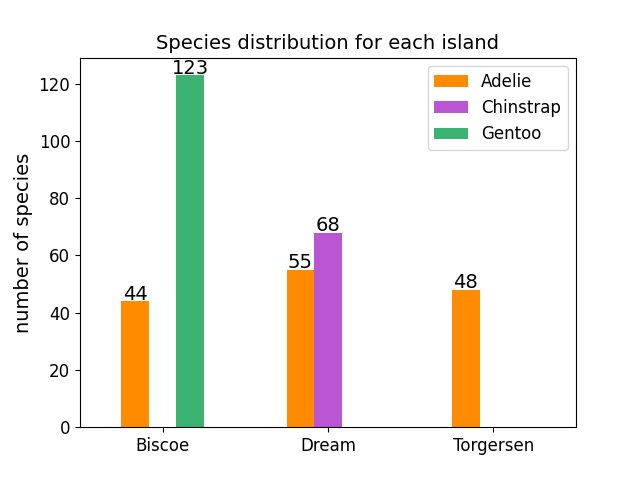
\includegraphics[width=0.48\textwidth]{islands.png} % Adjust the width as needed
  \caption{All numerical features show a significant statistical difference between the male and female measurements, as seen in the body mass boxplot above. Shown are median values, Q1 and Q3 quartiles, as well as outliers that are outside the range Q1-1.5IQR to Q3+1.5IQR, where IQR=Q3-Q1.}
  \label{fig:islands}
\end{wrapfigure}   

Two of these records can be deleted immediately as they are missing values for all of the numerical attributes and the sex feature and any imputation is unlikely to be reliable. The remaining nine records have no value only for the sex attribute. As can be seen in Figure~\ref{fig:islands}, the physical attributes of the male and female of each species are statistically different and so it is reasonable to consider assigning a sex to those records missing this attribute. Following standardization, a Shapiro-Wilk test was performed to confirm each numerical attribute exhibits a normal distribution [2] and Z-tests were performed to assess separately both the hypothesis that the missing sex value is male and that it is female [3]. It was found that two of the records could be imputed as male and three as female and these were then retained in the dataset. The remaining four records were removed from the dataset. The cleaned dataset consisted of 338 records made up of 147 Adelie penguins (74 male, 73 female), 68 Chinstrap penguins (34 male, 34 female) and 123 Gentoo penguins (62 male, 61 female).

A number of the methods applied in this work involve distance measures and so may be biased in favour of features with smaller standard deviations [4]. This bias can be removed by standardizing the four numerical attributes independently (to give zero mean and unity standard deviation). Standardization uses only the statistics of training sets, but standardization is also applied to test sets. If a dataset is imbalanced, AI approaches may be biased in predicting classes that are more commonly found in the training data. The Palmer penguin dataset is somewhat imbalanced, with the number of Chinstrap records being around half of that of either Adelie or Gentoo, which are present in similar numbers. The importance of imbalance depends on the analysis method applied. It is known that all the methods adopted in the current work are generally little affected by imbalanced data [5] and so no modifications were made to reduce imbalance.


Here is an example of an equation:
\begin{equation}
  \pi=4\left(1-\frac{1}{3}+\frac{1}{5}-\frac{1}{7}\ldots\right)
\end{equation}
or
\begin{equation}
  \pi=4\sum_{n=0}^\infty\frac{(-1)^{n}}{2n+1}
\end{equation}


where $\pi$ can be written in line by using \$'s. Here is a vector:
\begin{equation}
\mathbf{x}=\left(\begin{array}{c}x_1\\x_2\end{array}\right)
\end{equation}
You can write in \textbf{bold}, or \textsl{italics} or \texttt{true
  type}, often the latter is used for specific commands or libraries in a
programming language, as in `I used \texttt{numpy} v1.23.4 to\ldots'. Notice the use of the left quote symbol found in the top left of the keyboard to get the left quote. There is also blackboard bold often used for things like $\mathbb{R}$ for real numbers and there is calligraphic for fancy things like $\mathcal{L}$ but this is becoming increasing irrelevant to what you are likely to need! 







\end{document}
